\section{Examples of implementation of \littlunOne}

\subsection{Tables for \littlunOne and \littlunS}
\label{sec:sbox_tables}

\begin{figure}[ht]
\begin{minted}[breaklines]{c}
uint8_t littlun1_s4[16] =
        {0x0, 0xa, 0x4, 0xf, 0xc, 0x7, 0x2, 0x8,
         0xd, 0xe, 0x9, 0xb, 0x5, 0x6, 0x3, 0x1};
\end{minted}
\caption{The 4-bit S-box \littlunS used in \littlunOne as a \C array\label{tab4}}
\end{figure}

\begin{figure}[ht]
\begin{minted}[breaklines]{c}
uint8_t littlun1[256] =
        {0x00, 0x9b, 0xc2, 0x15, 0x5d, 0x84, 0x4c, 0xd1,
         0x67, 0x38, 0xef, 0xb0, 0x7e, 0x2b, 0xf6, 0xa3,
         0xb9, 0xaa, 0x36, 0x78, 0x2f, 0x6e, 0xe3, 0xf7,
         0x12, 0x5c, 0x9a, 0xd4, 0x89, 0xcd, 0x01, 0x45,
         0x2c, 0x63, 0x44, 0xde, 0x02, 0x96, 0x39, 0x70,
         0xba, 0xe4, 0x18, 0x57, 0xa1, 0xf5, 0x8b, 0xce,
         0x51, 0x87, 0xed, 0xff, 0xb5, 0xa8, 0xca, 0x1b,
         0xdf, 0x90, 0x6c, 0x32, 0x46, 0x03, 0x7d, 0x29,
         0xd5, 0xf2, 0x20, 0x5b, 0xcc, 0x31, 0x04, 0xbd,
         0xa6, 0x41, 0x8e, 0x79, 0xea, 0x9f, 0x68, 0x1c,
         0x48, 0xe6, 0x69, 0x8a, 0x13, 0x77, 0x9e, 0xaf,
         0xf3, 0x05, 0xcb, 0x2d, 0xb4, 0xd0, 0x37, 0x52,
         0xc4, 0x3e, 0x93, 0xac, 0x40, 0xe9, 0x22, 0x56,
         0x7b, 0x8d, 0xf1, 0x06, 0x17, 0x62, 0xbf, 0xda,
         0x1d, 0x7f, 0x07, 0xb1, 0xdb, 0xfa, 0x65, 0x88,
         0x2e, 0xc9, 0xa5, 0x43, 0x58, 0x3c, 0xe0, 0x94,
         0x76, 0x21, 0xab, 0xfd, 0x6a, 0x3f, 0xb7, 0xe2,
         0xdd, 0x4f, 0x53, 0x8c, 0xc0, 0x19, 0x95, 0x08,
         0x83, 0xc5, 0x4e, 0x09, 0x14, 0x50, 0xd8, 0x9c,
         0xf4, 0xee, 0x27, 0x61, 0x3b, 0x7a, 0xa2, 0xb6,
         0xfe, 0xa9, 0x81, 0xc6, 0xe8, 0xbc, 0x1f, 0x5a,
         0x35, 0x72, 0x99, 0x0a, 0xd3, 0x47, 0x24, 0x6d,
         0x0b, 0x4d, 0x75, 0x23, 0x97, 0xd2, 0x60, 0x34,
         0xc8, 0x16, 0xa0, 0xbb, 0xfc, 0xe1, 0x5e, 0x8f,
         0xe7, 0x98, 0x1a, 0x64, 0xae, 0x4b, 0x71, 0x85,
         0x0c, 0xb3, 0x3d, 0xcf, 0x55, 0x28, 0xd9, 0xf0,
         0xb2, 0xdc, 0x5f, 0x30, 0xf9, 0x0d, 0x26, 0xc3,
         0x91, 0xa7, 0x74, 0x1e, 0x82, 0x66, 0x4a, 0xeb,
         0x6f, 0x10, 0xb8, 0xd7, 0x86, 0x73, 0xfb, 0x0e,
         0x59, 0x2a, 0x42, 0xe5, 0x9d, 0xa4, 0x33, 0xc7,
         0x3a, 0x54, 0xec, 0x92, 0xc1, 0x25, 0xad, 0x49,
         0x80, 0x6b, 0xd6, 0xf8, 0x0f, 0xbe, 0x7c, 0x11};
\end{minted}
\caption{The \littlunOne S-box as a \C array\label{tab8}}
\end{figure}

\FloatBarrier

\subsection{SIMD software implementation of \littlunOne}
\label{sec:simdimplem}

In the context of 4 to 8-bit S-boxes, the Lai-Massey structure of the \littlun construction also allows to conveniently use ``vector'' Single Instruction Multiple Data (or SIMD) instructions for
efficient implementations. We discuss here an implementation of \littlunOne based mostly on the \pshufb instruction from Intel's SSSE3 instruction set.
%This instruction
%allows to perform 16 parallel lookups of a 4-bit S-box on a 128-bit register, which is particularly convenient to implement a similarly parallel application of
%a \littlun S-box on 128 bits. More precisely, the semantics of $x' \defas \pshufb~x~y$ can be defined as: 
%\[
%x'[i] \defas \left\{
%				\begin{array}{ll}
%				x[\lfloor y[i]\rfloor_4]  & \text{if the most significant bit of $y[i]$ is not set}\\
%				0 & \text{otherwise}
%				\end{array}
%	    \right.
%\]
%where $x$ and $y$ are vectors of 16 bytes.
The \pshufb instruction can easily be used in an implementation either by directly writing the relevant part of the program in assembler
or by using compiler intrinsics for a language such as \C. In the latter case, the intrinsic corresponding to the use of \pshufb is usually named \texttt{\_mm\_shuffle\_epi8}.
We give a small function implementing the \littlunOne S-box using \C intrinsics in \autoref{sse8}. Even without further tuning of the code, this function compares favourably with vector implementations
of other S-boxes in terms of efficiency. For instance, it needs about half the number of instructions of Hamburg's hand-written vector implementation of the \aes S-box \cite{vpaes}, although
this must be moderated by the fact that the AES S-box is cryptographically stronger.

\begin{figure}[ht]
\begin{minted}[breaklines]{c}
__m128i littlun_ps(__m128i x)
{
  __m128i xlo, xhi, xmid;

  __m128i LO_MASK = _mm_set1_epi8(0x0f);
  __m128i LO_SBOX = _mm_set_epi32(0x01030605, 0x0b090e0d, 0x0802070c, 0x0f040a00);
  __m128i HI_SBOX = _mm_set_epi32(0x10306050, 0xb090e0d0, 0x802070c0, 0xf040a000);

  xhi  = _mm_srli_epi16(x, 4);
  xhi  = _mm_and_si128(xhi, LO_MASK);
  xlo  = _mm_and_si128(x, LO_MASK);
  xmid = _mm_xor_si128(xlo, xhi);

  xmid = _mm_shuffle_epi8(LO_SBOX, xmid);
  xlo  = _mm_xor_si128(xlo, xmid);
  xhi  = _mm_xor_si128(xhi, xmid);

  xlo = _mm_shuffle_epi8(LO_SBOX, xlo);
  xhi = _mm_shuffle_epi8(HI_SBOX, xhi);
  x   = _mm_xor_si128(xlo, xhi);

  return x;
}
\end{minted}
\caption{Snippet for an SSE \C implementation of \littlunOne using compiler intrinsics.\label{sse8}}
\end{figure}

\FloatBarrier

\subsection{Hardware circuit for \littlunS}
\label{sec:circ}

\def\andGate{\begin{tikzpicture}[scale=0.5, circuit logic US]\node [and gate] {};\end{tikzpicture}}
\def\xorGate{\begin{tikzpicture}[scale=0.5, circuit logic US]\node [xor gate] {};\end{tikzpicture}}
\def\orGate{\begin{tikzpicture}[scale=0.5, circuit logic US]\node [or gate] {};\end{tikzpicture}}

\begin{figure}[ht]
\begin{center}
%\begin{turn}{-90}
%\begin{minipage}{4.5cm}
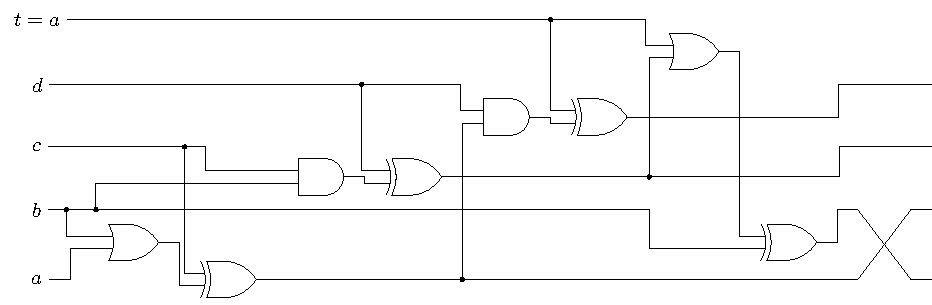
\includegraphics[scale=0.75]{../II_LOTF/littlun/sb4c.pdf}
%\end{minipage}
%\end{turn}
\end{center}
\caption[A circuit implementation of \littlunS.]{A circuit implementation of \littlunS. 
The symbols~\protect\andGate,~\protect\orGate~and~\protect\xorGate~represent the AND,
OR and XOR gates respectively.\label{sb4_circ}}
\end{figure}

\FloatBarrier
